\documentclass{report}
\usepackage[utf8]{inputenc}
\usepackage[T1]{fontenc}
\usepackage[frenchb]{babel}
\usepackage{amsmath,amsfonts,graphicx}

\usepackage{textcomp}
\usepackage{tgpagella}

\usepackage{algpseudocode}

\newcommand{\norm}[1]{\left\lVert#1\right\rVert}

\newcommand{\icol}[1]{% inline column vector
  \left(\begin{matrix}#1\end{matrix}\right)%
}
\newcommand{\irow}[1]{% inline row vector
  \begin{matrix}(#1)\end{matrix}%
}

\title{Notes d'avancement}
\author{Arnaud Bletterer}
\date{\today}

\graphicspath{{Figures/}}

\begin{document}

\maketitle

\chapter{Visualisation de nuages de points massifs}

La visualisation de sites archéologiques, de monuments historiques issus d'acquisition 3D pose un problème en termes de taille des données.
En effet, il y a tellement d'échantillons qui ont été acquis qu'il est impossible de les faire rentrer dans la mémoire de la carte graphique.
De ce fait, il est nécessaire de trouver des méthodes intelligentes de décimation, avant d'appliquer le moindre algorithme de visualisation.
La question qui se pose alors est "Mais comment décimer facilement et de manière efficace cette donnée?"

Il est essentiel de trouver des solutions intelligentes afin d'optimiser la visualisation de telles primitives.

\chapter{Idées} % (fold)
\label{cha:idees}

\section{Synthèse de cartes de profondeurs}

Etant donné qu'il n'est pas possible d'obtenir des cartes de profondeur pour chaque nuage de points ou objet virtuel (donnée acquise différemment, ou donnée d'origine non disponible), il faut obtenir un moyen de les synthétiser.
Ca permet de ne pas limiter la méthode aux cartes de profondeurs fournies par les scanners, mais d'offrir un moyen de la générer de manière simple afin d'utiliser la méthode sur plus de données différentes (dans le même esprit que \cite{Sor11}).

Pourquoi ne pas simplement faire un rendu de profondeur comme pour les maillages?

Une carte de profondeur correspond à un échantillonnage de la surface visible d'un objet réel. Certains points sont cachés du fait de la forme de l'objet et de la position/rotation de la caméra au moment de l'acquisition. Lors d'acquisitions réelles, les points obtenus et présents sur la carte de profondeur sont forcément les points qui étaient visibiles au moment de l'acquisition, car c'est de cette manière que le mécanisme d'acquisition fonctionne (sauf pour la tomographie).
Afin de reproduire ce phénomène lors de rendus de synthèse, il faut définir la profondeur des points de la scène.
Cette donnée est fournie par ce qu'on appelle le \textbf{z-buffer} (OpenGL). Ce z-buffer est un tampon qui stocke pour chaque pixel de la zone de rendu, la profondeur du point acquis dans cette zone. Si un autre point se projette sur un même pixel, on compare la profondeur des 2 points, et on garde celui dont la profondeur est la plus faible (il est plus près de la caméra).
Cette façon de faire est fortement utilisée sur les maillages polygonaux, car définie de manière implicite au moment de la rastérisation dans le pipeline de rendu. L'algorithme ne fait pas la différence entre un sommet et un point faisant partie d'une face, car il considére l'objet rendu comme une unique surface.
Mais pour les nuages de points, c'est différent. En effet, ceux-ci ne définissent pas d'autres primitives que les points (pas d'arêtes, ni de faces).
Ce qui fait qu'au moment de la rastérisation, il y a beaucoup de chance pour qu'un point du fond se projette sur un pixel différent de points plus près de la caméra.

Néanmoins il existe des méthodes permettant de générer des cartes de profondeur à partir de nuages de points.
Dans \cite{}, un outil mathématique est défini. L'idée est de projeter l'ensemble des points par rapport à un cercle donné, et de regarder les points faisant parti de l'enveloppe convexe du nuage de points, il s'agit des points actuellement visible.
Le centre du cercle correspond à la position de la caméra au moment du rendu, et sa taille est donnée en paramètre.
Un paramètre trop petit fera apparaître plus de points que nécessaires (faux positifs).
Un paramètre trop grand cachera des parties visibles de l'objet (faux négatifs).

Dans \cite{} l'idée est d'éliminer les faux positifs (points de l'espace projetés sur l'espace écran qui ne font pas partie de la surface visible) après une projection classique. Pour cela, ils utilisent une notion de visibilité basée sur la taille d'un cone dont le sommet est le point courant, et la largeur du cone est définie de façon à ce que le cone soit tangent aux points adjacents au point courant (adjacence définie grâce à la connectivité implicite dans l'espace écran).
Si l'angle d'ouverture du cone est supérieur à un paramètre donné, alors le point est considéré comme visible, sinon le point est considéré comme ne faisant pas partie de la surface visible.

\section{Sur-échantillonnage du nuage de points}

En général, les acquisitions numériques d'un objet réel sont nombreuses, afin d'acquérir le maximum de détails sur l'objet numérisé.
De ce fait, il y a énormément de zones "sur-échantillonnées" (qui sont vues par plus d'une caméra, et donc, par définition, échantillonnées par plus d'une carte de profondeur).

\section{Suppression de la redondance}

Dans l'idée d'utiliser les cartes de profondeur comme support de remplacement des nuages de points, il parait évident de supprimer la \textbf{redondance} (zone de l'espace où l'information géométrique est stockée par plusieurs cartes de profondeur à la fois).
Pour se faire, il faut dans un premier temps trouver les zones qui sont vues par plusieurs caméras à la fois.

\subsection{Identification des zones vues par plusieurs caméras}

On dit qu'une zone est vue par plusieurs caméras si la projection des points d'une zone du nuage de points se fait sur plusieurs cartes de profondeur.
Pour détecter ces zones, une méthode consiste à projeter les points associés à une caméra sur chacune des autres caméras.
De cette façon, on peut rapidement appairer des paires de points entre elles.
Une méthode efficace consiste à simuler des rendus de synthèse, en décidant de visualiser les points d'une carte, par rapport à une autre caméra.
On en obtient une autre carte de profondeur, et les zones des deux cartes qui sont similaires sont considérées comme représentant le même point.

\subsection{Suppression des zones sur-échantillonnées}

Une fois qu'un appairage de points a été effectué, il faut définir une métrique afin de sélectionner les points à conserver, et ceux à supprimer.

Une première, simple à appliquer, consiste à garder les zones les mieux échantillonnées.
Pour cela, il suffit de comparer la direction de vue d'une caméra (vecteur orthogonal au plan caméra) avec la normale en chacun des points issus du plongement de la carte de profondeur associée à cette caméra.
Un simple produit scalaire $\theta_p = \vec{n_c} \cdot \vec{n_p}$ permet d'obtenir une valeur $\theta_p \in [0,1]$ qui distingue les zones bien échantillonées (produit scalaire fort) des zones moins bien échantillonnées (produit scalaire faible).

\begin{figure}[h]
\centering
	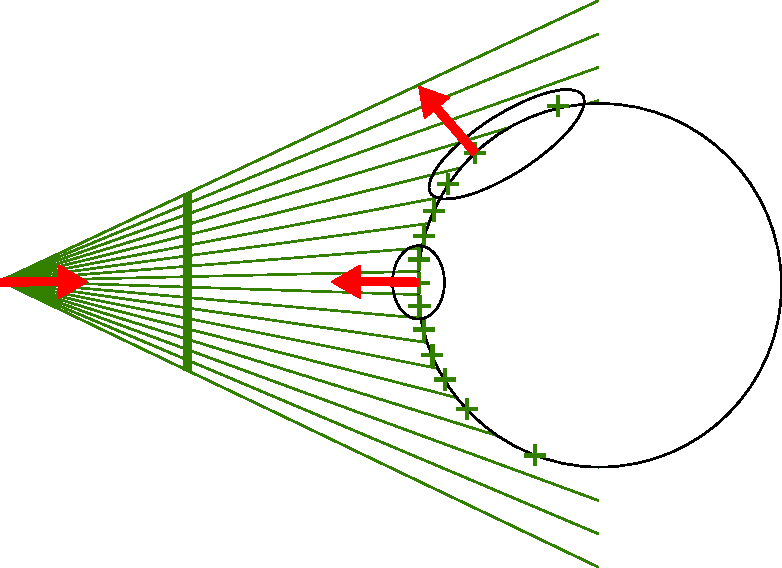
\includegraphics[scale=0.5]{GoodVisibility-Normals}
	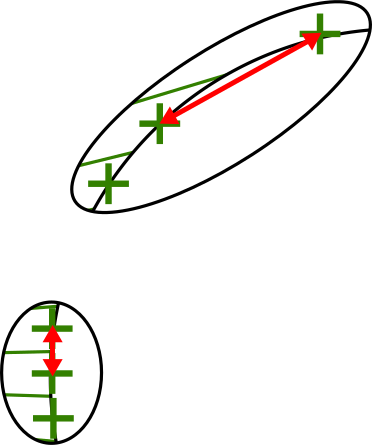
\includegraphics[scale=0.4]{GoodVisibility-Zoom}
	\caption{Estimation du l'échantillonnage de la carte de profondeur en comparant l'alignement des normales en chacun des points avec }
\end{figure}

Une autre métrique pourrait représenter la densité de points présents dans une zone.
En effet, la connectivité implicite de la carte de profondeur permet de faciliter les requêtes de voisinage au sein d'une même carte (et même entre plusieurs cartes).
Du coup, une idée serait de regarder la densité d'échantillonnage dans l'espace 3D parmi un voisinage de points sur la carte de profondeur.

Pour se faire, un méthode simple consiste à regarder le nombre de points provenant de la même carte de profondeur qui appartiennent à la sphère de rayon $r$ centrée un chacun des points de la carte de profondeur. En divisant le nombre points trouvés par le volume de la sphère :

\begin{equation}
	\theta_p = \frac{n}{\frac{4\pi r^3}{3}}
\end{equation}

\begin{figure}[h]
\centering
	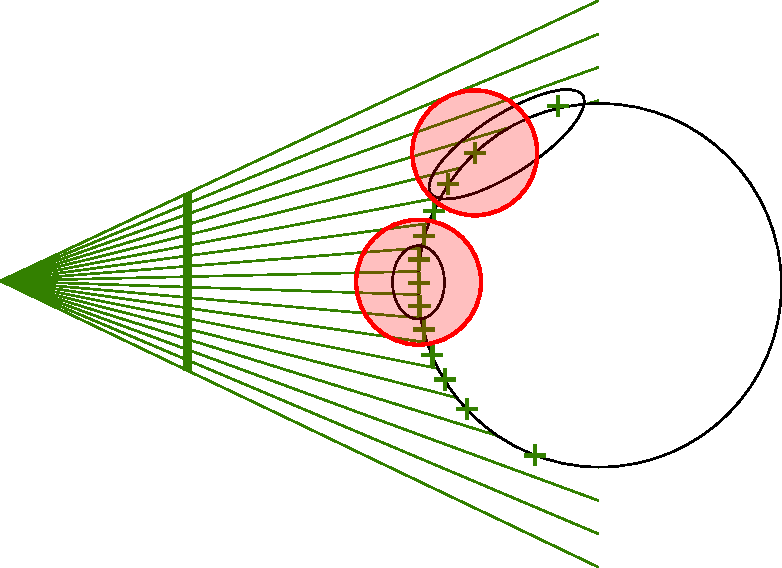
\includegraphics[scale=0.5]{GoodVisibility-Density}
	\caption{Estimation du l'échantillonnage de la carte de profondeur en un point particulier}
\end{figure}

\subsection{Calcul de normales}

La normale a la surface peut être facilement obtenue, à condition de connaître le voisinage exact d'un point sur la surface.
En utilisant le 4-voisinage d'un point, on peut facilement obtenir les 2 vecteurs définissant le plant tangent à la surface en ce point.
La normale s'obtient donc facilement comme étant le produit vectoriel entre ces deux vecteurs $\vec{n_p} = \vec{u_p} \times \vec{v_p}$

\section{Traitement du nuage de points}

Etant donné qu'une carte de profondeur est une image (paramétrisation discrète régulière), une idée serait d'appliquer des algorithmes venant du traitement des images (un domaine qui est activement étudié depuis une cinquantaine d'années) afin de modifier la géométrie du nuage de points.

\subsection{Représentation multi-résolution}

Un exemple simple correspond à l'utilisation d'une transformée en ondelettes (méthode de décomposition d'un signal en un ensemble de signaux "hautes-fréquence" et "basse-fréquence"). En appliquant une transformée en ondelettes par carte de profondeur, on définit une hiérarchie de niveaux de résolution sur chacune des cartes de profondeur.
En plongeant dans l'espace 3D les pixels de toutes les cartes de profondeur à un certain niveau de résolution, on peut visualiser un nuage de points simplifié.

\subsection{Compression des données}

Des algorithmes très efficaces de compression des données ont été développés, en particulier dans le cadre de la compression d'images.
On peut distinguer ces algorithmes en deux familles distinctes :
\begin{itemize}
	\item Sans perte (lossless) :
	Ces méthodes de compression permettent, comme leur nom l'indique, de compresser les données sans perdre la moindre information (il est possible de reconstruire parfaitement le signal original). Ces méthodes permettent d'appliquer une compression moins fortes que celles de la prochaine famille, néanmoins sont très utiles dans certaines applications où la préservation des données est essentielle.
	\item Avec perte (lossy) :
	Ces méthodes ont été développées dans le but d'augmenter le ratio de compression. L'idée de départ a été de se dire que les données de bases contenaient plus d'informations que nécessaires, et qu'il était possible de perdre de l'information sans pour autant qu'aucune dégradation des données ne soient visibles pour les humains.
	Partant de ce postulat, des méthodes on été développées afin de quantifier les données avant compression (quantification = représentation d'un signal continu par un ensemble de valeurs discrètes). Le pas de quantification choisi influe donc sur le débit obtenu après compression.
\end{itemize}

Tout l'objectif de la compression se résume au fait de pouvoir reconstruire un signal le plus fidèlement possible, en ayant le débit le plus faible possible. C'est à dire en ayant le moins d'information à stocker.

Concernant notre application précise, l'idée est de compresser le nuage de points en le conservant sous la forme de cartes de profondeur, et d'utiliser des algorithmes ayant prouvé leur efficacité en traitement des images, afin de compresser le nuage de points de manière efficace.

Cette approche est très originale. En effet, dans l'état de l'art des méthodes de compression des nuages de points, un des principaux problèmes correspond au manque de structuration dans le nuage de points, ce qui fait qu'il est difficile de compresser ces données de manière efficace de manière directe.
Les méthodes développées se sont donc intéressées à la création de structures représentant le nuage de points, et de ne pas compresser le nuage de points, mais la structure nouvellement créée.

Cependant aucun de ces travaux ne s'intéresse à l'origine des nuages de points (données obtenues directement à la sortie des scanners 3D). Parce qu'au moment de l'acquisition, les données sont structurées.
Après chaque acquisition, une paramétrisation est obtenue (sous la forme d'une carte de profondeur par exemple), et cette paramétrisation est une représentation structurée du nuage de points. Alors pourquoi ne pas se servir des cartes de profondeur directement pour faire la compression dessus?

Nous avons décidé d'utiliser l'algorithme JPEG2000 dans un premier temps, qui est un des plus utilisés concernant la compression d'images sans perte.

Une implémentation de l'algorithme était déjà disponible dans MATLAB, nous avons donc choisi d'utiliser celle-ci pour commencer.

\section{Erreur géométrique} % (fold)

\subsection{Erreur d'échantillonnage d'une surface} % (fold)

\subsection{Erreur de suppression des zones redondantes}

Au moment de supprimer les zones redondantes, le but recherché est de supprimer des zones "sur-échantillonnées" (vues depuis des caméras placées à des points de vue différents).
Ces zones contiennent plus de données que nécessaires pour représenter un nuage de points, et il n'est pas utile de garder tous les points dans cette zone afin de représenter la même surface sous-jacente.

Etant donné que plusieurs critères s'offrent à nous concernant la suppression de ces zones "sur-échantillonnées", nous devons sélectionner le meilleur, en ne considérant pas uniquement un critère qualitatif, mais surtout quantitatif. Pour se faire, nous devons comparer le nuage de points original, avec les nuages de points obtenus après suppression de la redondance.

\subsection{Erreur de quantification} % (fold)

Afin d'obtenir un taux de compression plus important, on peut quantifier les coefficients d'ondelettes obtenus, afin de représenter les valeurs de profondeur sur moins de 24 bits (valeurs de base).
En général, on définit un modèle d'allocation de bits. Ce modèle est une méthode itérative qui en fonction de la demande en entrée (débit total ou erreur géométrique), va adapter la quantification appliquée pour approcher au mieux la demande en entrée (minimiser l'erreur géométrique pour un débit donné, et minimiser le débit pour une erreur géométrique donnée)

Et pour représenter de manière quantitative l'impact de la quantification sur la perte de données, il est nécessaire d'utiliser une métrique de distance entre un nuage de points $M$ et ce même nuage quantifié $\hat{M}$.
Une manière simple de représenter l'impact de la quantification consiste à regarder l'erreur quadratique moyenne entre les deux nuages, en comparant les points 1 à 1 entre la position d'un point avant et après quantification:

\begin{equation}
	MSE_{geom} = \frac{1}{N}\sum_i^N\norm{X_i-\hat{X}_i}^2 \label{eq:mse_geom},
\end{equation}

où $N$ représente le nombre de points composant le nuage, $X_i$ et $\hat{X}_i$ un point avant et après quantification, respectivement.
Cette expression considère la position des points dans l'espace, mais il est possible d'obtenir cette position à partir des données d'une carte de profondeur :

\begin{equation}
	X_{c_k} = \icol{x_{c_k}'\\y_{c_k}'\\z_{c_k}'} = R_c^{-1}A_c^{-1}\icol{x_{c_k}\\y_{c_k}\\1}z(x_{c_k},y_{c_k})+T_c,
\end{equation}

où $R_c$ et $T_c$ représentent la matrice de rotation et le vecteur de translation correspondant aux paramètres extrinsèques de la caméra $c$, et $A_c$ la matrice de projection correspondant aux paramètres intrinsèques de la caméra.

La différence entre $X$ et $\hat{X}$ peut donc s'écrire :

\begin{align}
	\icol{x_{c_k}'\\y_{c_k}'\\z_{c_k}'} - \icol{\hat{x}_{c_k}'\\\hat{y}_{c_k}'\\\hat{z}_{c_k}'}
	&= \Big(R_c^{-1}A_c^{-1}\icol{x_{c_k}\\y_{c_k}\\1}z(x_{c_k},y_{c_k})+T_c \Big) - \Big(R_c^{-1}A_c^{-1}\icol{x_{c_k}\\y_{c_k}\\1}\hat{z}(x_{c_k},y_{c_k})+T_c \Big) \\
	&= \Big(R_c^{-1}A_c^{-1}\icol{x_{c_k}\\y_{c_k}\\1}z(x_{c_k},y_{c_k}) \Big) - \Big(R_c^{-1}A_c^{-1}\icol{x_{c_k}\\y_{c_k}\\1}\hat{z}(x_{c_k},y_{c_k}) \Big) \\
	&= R_c^{-1}A_c^{-1}\icol{x_c\\y_c\\1}\Big(z(x_c,y_c)-\hat{z}(x_c,y_c)\Big) \label{eq:diff_img}.
\end{align}

En remplaçant \eqref{eq:diff_img} dans \eqref{eq:mse_geom}, on obtient :

\begin{align}
	MSE_{geom_c} &= \frac{1}{N}\sum_i^N\norm{R_c^{-1}A_c^{-1}\icol{x_{c_i}\\y_{c_i}\\1}\Big(z(x_{c_i},y_{c_i})-\hat{z}(x_{c_i},y_{c_i})\Big)}^2 \\
	&= \frac{1}{N}\sum_i^N\norm{R_c^{-1}A_c^{-1}\icol{x_{c_i}\\y_{c_i}\\1}}^2\Big(z(x_{c_i},y_{c_i})-\hat{z}(x_{c_i},y_{c_i})\Big)^2
\end{align}

De cette manière, il est possible de mesurer l'erreur géométrique directement à partir des valeurs de profondeurs dans les cartes de profondeur.

\subsection{Calcul d'erreur géométrique à partir de valeurs d'intensité}

Soit $a = (x,y,z)$ un point de l'espace et $b = (wx,wy,wz,w)$ sa représentation en 3D homogène. On peut écrire la norme $L^2$ de $a$ à partir de $b$ :

\begin{equation}
	\norm{a}_2^2 = \frac{\norm{b}_2^2}{w^2}-1.
\end{equation}

Etant donné que $b$ peut être exprimé comme le plongement d'un pixel d'une carte de profondeur grâce à la matrice de plongement $M^{-1}$ associée à cette carte de profondeur :

\begin{equation}
	b = M^{-1}c,
\end{equation}

on peut exprimer la norme $L^2$ de $a$ à partir des valeurs de $c$ :

\begin{equation}
	\norm{a}_2^2 = \frac{\norm{M^{-1}c}^2}{w^2}-1,
\end{equation}

où $w$ est le résultat du produit scalaire entre la dernière ligne de $M^{-1}$ et du vecteur $c$ :

\begin{equation}
	w = M_4^{-1}\cdot c.
\end{equation}

\chapter{Visualisation}

\section{A partir de cartes de profondeur}

Un des objectifs que nous avons consiste à nous défaire complètement de la représentation classique des nuages de points (tableau de coordonnées 3D), et de travailler directement avec les données issues des cartes de profondeur + matrices de projection (étant donné que les représentations sont équivalentes).

Nous avons donc implémenté un premier pas dans cette direction, où un nuage de points est reconstruit à partir de cartes de profondeur uniquement.
Pour se faire, nous générons un VBO à la volée, en plongeant les points contenus dans les différentes cartes de profondeur, grâce aux matrices de projection.
Cette création est faite sur GPU, dans un Compute Shader, ce qui rend la création de ces structures de données très rapide (< 1s).
Après que le VBO soit créé, la visualisation se fait de façon traditionnelle.

Maintenant que nous savons faire cela, une deuxième étape consisterait à décompresser les cartes de profondeur sur GPU avant de générer le VBO.
Pour se faire, il faut connaître l'algorithme utilisé pour compresser les images. Ce qui rend plus délicate l'utilisation de JPEG2000, sachant la difficulté d'implémentation de cet algorithme.

Une autre solution consiste à faire un codeur "maison", en choisissant l'ondelette la plus appropriée, et en quantifiant nous-même les coefficients d'ondelettes.
Etant donné que l'opération de transformation est fortement parallélisable (tous les traitements sont réalisés sur chaque pixel indépendamment), il suffirait d'écrire un décodeur dans le GPU (un "Compute Shader" par exemple), afin de pouvoir transmette la donnée compressée au GPU, et limiter les échanges entre CPU et GPU.

\subsection{Sous-échantillonnage}
\label{subs:sous_echantillonnage}

En appliquant une transformée en ondelettes non liftée et en visualisant le nuage de points à partir de la reprojection des cartes de profondeur à différentes résolutions, nous visualisons un sous-échantillonnage régulier, par morceaux, du nuage de points.

Il serait intéressant de pouvoir sous-échantillonner ce nuage de points de manière non-régulière, en effectuant un échantillonnage en disque de poisson par exemple, préservant des propriétés dites de "bruit bleu"

\subsubsection{Bruit bleu}
\label{subs:Bruit_bleu}

Le bruit bleu est une couleur de bruit qui a une densité spectrale proportionelle à sa fréquence.
Cela signifie que la puissance et l'énergie du signal augmente en même temps que la fréquence.
Ce type de bruit connait un fort intérêt en Informatique Graphique, étant donné que son utilisation permet d'éviter des effets d'aliasing lors de différents rendus, lorsque la densité de points projetés sur l'écran devient trop importante.
La donnée étant sous-échantillonnée, il est fort courant de se retrouver avec des effets de "repliement de spectre", donnant l'impression de motifs dessinés à l'écran, bien que la donnée ne contienne aucun dessin de ce genre.

Ce problème de repliement de spectre est dû au non respect du théorème d'échantillonnage de Nyquist Shannon.

\chapter{Reconstruction de surface}

Etant donné que les processeurs graphiques sont optimisés pour le traitement de géométrie discrète sous la forme de triangles, il est naturel de se tourner vers ce genre de représentation lorsque le nombre de primitives à visualiser devient important.

Une des méthodes les plus utilisées pour reconstruire la topologie sous-jacente à un ensemble d'échantillons est ce qu'on appelle les "diagrammes de Voronoi".

\section{Diagramme de Voronoï}

\subsection{Diagramme de Voronoï basique}

Un diagramme de Voronoï est une structure de données représentant une partition d'un espace de dimension $d$ $E^d$.
A partir d'un ensemble de $k$ sites, l'idée est de trouver pour chaque site la zone de l'espace la plus proche de ce site.
Concrètement, il s'agit de définir, pour chaque point de l'espace $p$ de quel site $k$ il est le plus proche :

\begin{equation}
  \{p \in E^d \mid d(k_i, p) < d(k_j, p), \forall j \neq i\},
\end{equation}

où $d(k,p)$ correspond à la distance entre le site $k$ et le point $p$. Cette fonction de distance peut par exemple correspondre à la distance euclidienne (norme l2) :

\begin{equation}
  \norm{k-p} = \sqrt{\sum_i^d (k_i-p_i)^2}
\end{equation}

\subsection{Diagramme de Voronoï pondéré}

\bibliographystyle{plain}
\bibliography{bibliography.bib}

\end{document}
